% !TEX root = ../main.tex

\clearpage
% Source PDF page 23.
\section{第八章\quad 奶蛙周边的售卖壮大}

随着奶蛙的爆火，紧随抽象潮流的商家们也纷纷上架奶蛙周边。~(见\figref{fig:08-1})

% !TEX root = ../../main.tex
\begin{figure}[H]
  \centering
  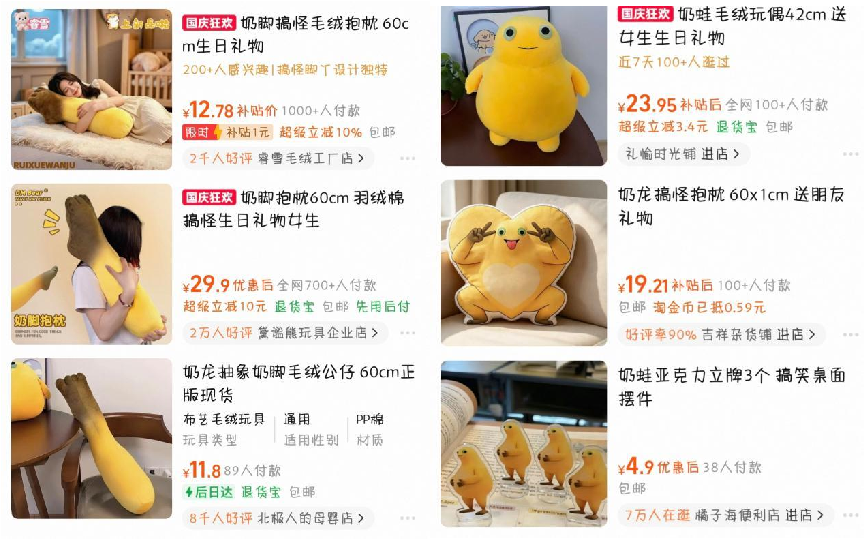
\includegraphics[width=352.85bp,height=0.76\textheight,keepaspectratio]{figures/chapter08/figure08_1.pdf}
  \renewcommand{\thefigure}{8.1}
  \caption{淘宝售卖的奶脚抱枕（左）和奶蛙玩偶、亚克力等（右）}
  \label{fig:08-1}
\end{figure}


% !TEX root = ../../main.tex
\begin{figure}[H]
  \centering
  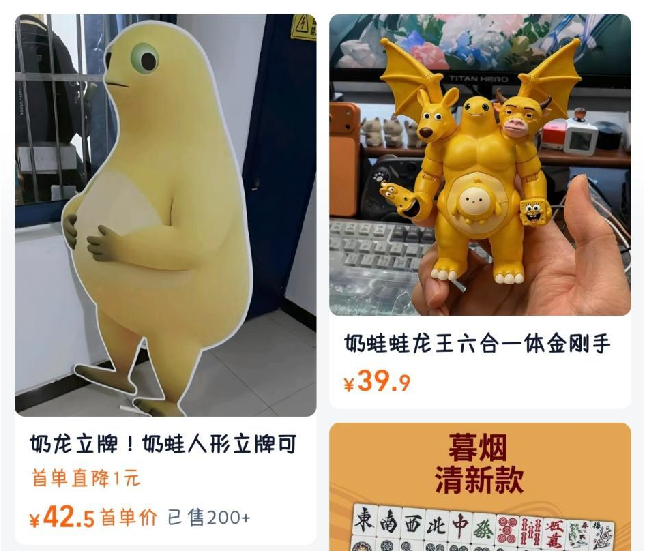
\includegraphics[width=263.3bp,height=0.76\textheight,keepaspectratio]{figures/chapter08/figure08_2.pdf}
  \renewcommand{\thefigure}{8.2}
  \caption{淘宝售卖的 2m 奶蛙人形立牌和奶蛙六合一战神金刚}
  \label{fig:08-2}
\end{figure}


其中最具有影响力的，无疑是奶蛙立牌。各个高校的奶家人不约而同有了一个大胆的想法...我们将会在第九章中具体展开。~(见\figref{fig:08-2})

其中有一些产品无疑是具有新意和实用或观赏价值的。我们将会稍微提及一些有趣的奶味产品。

\clearpage
% Source PDF page 24.
这是淘宝上售卖的奶蛙抽纸盒，由 3D 打印技术制作而成。简单的工艺，不简单的创意。口吐白纸的奶蛙正是笑到极点的表现。~(见\figref{fig:08-3})

% !TEX root = ../../main.tex
\begin{figure}[H]
  \centering
  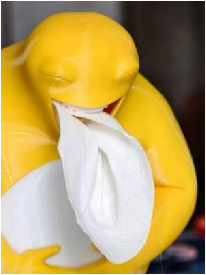
\includegraphics[width=83.98bp,height=0.76\textheight,keepaspectratio]{figures/chapter08/figure08_3.pdf}
  \renewcommand{\thefigure}{8.3}
  \caption{奶蛙抽纸盒}
  \label{fig:08-3}
\end{figure}


这是淘宝上售卖的奶味创意奶夜灯，巧妙地运用了阴影的效果，让奶蛙以两种姿态出现在奶民们夜晚的床头。当你夜不能寐的时候，还有奶灯温馨伴你左右。~(见\figref{fig:08-4})

% !TEX root = ../../main.tex
\begin{figure}[H]
  \centering
  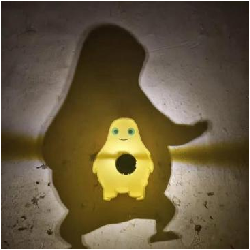
\includegraphics[width=102.03bp,height=0.76\textheight,keepaspectratio]{figures/chapter08/figure08_4.pdf}
  \renewcommand{\thefigure}{8.4}
  \caption{创意奶夜灯，阴影呈现奶蛙的架势}
  \label{fig:08-4}
\end{figure}


这是淘宝上售卖的奶勺子，巧妙地把舌头的形状和勺子联系起来，颇有形体美。\sout{弥补了不能和奶蛙舌吻的遗憾（划去）。}~(见\figref{fig:08-5})

% !TEX root = ../../main.tex
\begin{figure}[H]
  \centering
  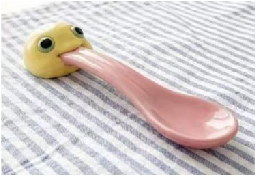
\includegraphics[width=104.38bp,height=0.76\textheight,keepaspectratio]{figures/chapter08/figure08_5.pdf}
  \renewcommand{\thefigure}{8.5}
  \caption{创意奶勺子}
  \label{fig:08-5}
\end{figure}


这是某网购平台上售卖的奶内裤。嗯...有点太神圣了。~(见\figref{fig:08-6})

% !TEX root = ../../main.tex
\begin{figure}[H]
  \centering
  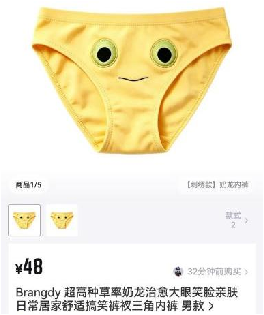
\includegraphics[width=107.75bp,height=0.76\textheight,keepaspectratio]{figures/chapter08/figure08_6.pdf}
  \renewcommand{\thefigure}{8.6}
  \caption{创意奶内衣}
  \label{fig:08-6}
\end{figure}


\clearpage
% Source PDF page 25.
这是某大学图书馆内的奶蛋椅。学完《奶概》之后惬意地往里面一坐，感觉奶蛙的笑声仿佛回响在耳边一样。~(见\figref{fig:08-7})

% !TEX root = ../../main.tex
\begin{figure}[H]
  \centering
  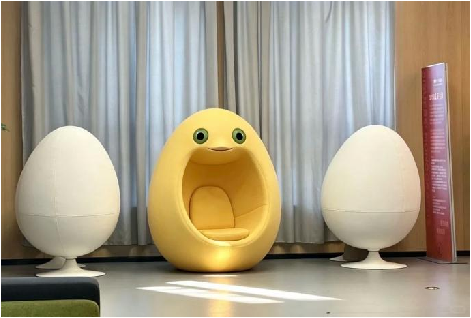
\includegraphics[width=192bp,height=0.76\textheight,keepaspectratio]{figures/chapter08/figure08_7.pdf}
  \renewcommand{\thefigure}{8.7}
  \caption{创意奶蛋椅}
  \label{fig:08-7}
\end{figure}


这是淘宝上售卖的奶蛙假面。戴上它来成为社交悍匪。~(见\figref{fig:08-8})

% !TEX root = ../../main.tex
\begin{figure}[H]
  \centering
  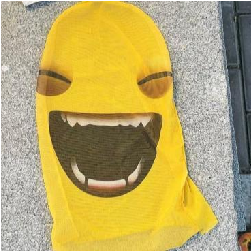
\includegraphics[width=102.85bp,height=0.76\textheight,keepaspectratio]{figures/chapter08/figure08_8.pdf}
  \renewcommand{\thefigure}{8.8}
  \caption{奶蛙假面}
  \label{fig:08-8}
\end{figure}


这是淘宝上售卖的奶蛙小抱枕。带着小奶蛙周游世界吧。~(见\figref{fig:08-9})

% !TEX root = ../../main.tex
\begin{figure}[H]
  \centering
  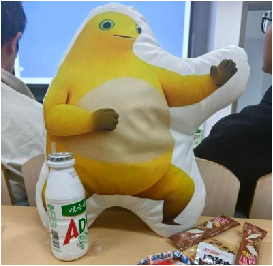
\includegraphics[width=111.52bp,height=0.76\textheight,keepaspectratio]{figures/chapter08/figure08_9.pdf}
  \renewcommand{\thefigure}{8.9}
  \caption{奶蛙小抱枕}
  \label{fig:08-9}
\end{figure}


这是淘宝上售卖的奶蛋小摆件。搭建你自己的奶蛋大军吧！~(见\figref{fig:08-10})

% !TEX root = ../../main.tex
\begin{figure}[H]
  \centering
  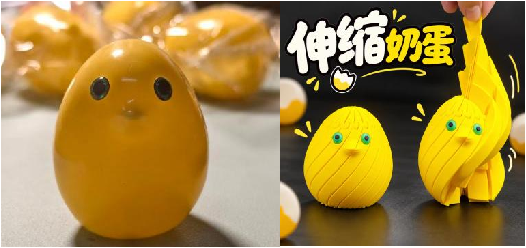
\includegraphics[width=214.74bp,height=0.76\textheight,keepaspectratio]{figures/chapter08/figure08_10.pdf}
  \renewcommand{\thefigure}{8.10}
  \caption{塑料奶蛋小摆件（左）与伸缩奶蛋解压玩具（右）}
  \label{fig:08-10}
\end{figure}


